\documentclass[compress]{beamer}

\mode<presentation>
{
  %\usetheme{Warsaw}
  %\usecolortheme{spruce}
  % or ...
	%\useoutertheme{infolines}
  %\setbeamercovered{transparent}
  
  \usetheme{CambridgeUS}
    \setbeamercolor{item projected}{bg=darkred}
    \setbeamertemplate{enumerate items}[default]
    \setbeamertemplate{navigation symbols}{}
    \setbeamercovered{invisible}
    \setbeamercolor{block title}{fg=darkred}
    \setbeamercolor{local structure}{fg=darkred}
  
  % or whatever (possibly just delete it)
}

\usepackage{verbatim} 
\usepackage{listings}
\usepackage{tikz}
\usetikzlibrary{arrows.meta}
\usetikzlibrary{shapes}
\tikzstyle{block}=[draw opacity=0.7,line width=1.4cm]

\definecolor{darkgreen}{RGB}{50,171,24}

\newcommand{\bigpause}{\bigskip \pause}

\lstloadlanguages{C++}
\lstnewenvironment{code}
	{%\lstset{	numbers=none, frame=lines, basicstyle=\small\ttfamily, }%
	 \csname lst@SetFirstLabel\endcsname}
	{\csname lst@SaveFirstLabel\endcsname}
\lstset{% general command to set parameter(s)
	language=C++, basicstyle=\footnotesize\sffamily, keywordstyle=\slshape,
	emph=[1]{tipo,usa}, emphstyle={[1]\sffamily\bfseries},
	basewidth={0.47em,0.40em},
	columns=fixed, fontadjust, resetmargins, xrightmargin=5pt, xleftmargin=15pt,
	flexiblecolumns=false, tabsize=2, breaklines,	breakatwhitespace=false, extendedchars=true,
	numbers=left, numberstyle=\tiny, stepnumber=1, numbersep=9pt,
	frame=l, framesep=3pt,
}

\usepackage[spanish]{babel}
% or whatever

\usepackage[utf8]{inputenc}
% or whatever

\usepackage{times}
\usepackage[T1]{fontenc}
% Or whatever. Note that the encoding and the font should match. If T1
% does not look nice, try deleting the line with the fontenc.


\title[Camino mínimo en grafos] % (optional, use only with long paper titles)
{Camino mínimo en grafos}

\author[Melanie Sclar] % (optional, use only with lots of authors)
{~Melanie Sclar}
% - Give the names in the same order as the appear in the paper.
% - Use the \inst{?} command only if the authors have different
%   affiliation.
\institute[UBA] % (optional, but mostly needed)
{
  %\inst{1}%
  Facultad de Ciencias Exactas y Naturales\\
  Universidad de Buenos Aires
}
\date[Nacional OIA 2016] % (optional, should be abbreviation of conference name)
{Nacional OIA 2016}

% Ac¿ se puede insertar el logo de la UBA
% \pgfdeclareimage[height=0.5cm]{university-logo}{university-logo-filename}
% \logo{\pgfuseimage{university-logo}}



% Delete this, if you do not want the table of contents to pop up at
% the beginning of each subsection:
\AtBeginSubsection[]
{
  \begin{frame}<beamer>{Contenidos}
    \tableofcontents[currentsection,currentsubsection]
  \end{frame}
}

\newcommand{\be}{\begin{equation*}}
\newcommand{\ee}{\end{equation*}}
\newcommand{\state}[1]{\left|\,#1\,\right\rangle}
\newcommand{\costate}[1]{\left\langle\,#1\,\right|}
\newcommand{\trace}{\text{Tr}}
\newcommand{\su}{\uparrow}
\newcommand{\sd}{\downarrow}
\newcommand{\im}{\text{Im}}
\newcommand{\re}{\text{Re}}

% If you wish to uncover everything in a step-wise fashion, uncomment
% the following command:

%\beamerdefaultoverlayspecification{<+->}


\begin{document}
\pgfdeclarelayer{background}
\pgfsetlayers{background,main}
\begin{frame}
  \titlepage
\end{frame}

\section{Camino mínimo}
\subsection{Introducción}
\begin{frame}
Esta charla tratará sobre uno de los problemas más renombrados de la
computación: \textbf{el problema del camino mínimo}. Este problema 
consiste en hallar la mejor forma de ir desde un punto a otro (o a varios
otros) minimizando la distancia recorrida, el tiempo invertido, entre
varias posibilidades.

\bigskip
\bigskip

Es un problema muy útil en las olimpíadas, pero no solamente aquí.
Veamos dos ejemplos de la vida real que deben resolver el problema que
trataremos hoy.
\end{frame}


\begin{frame}{Camino m\'inimo}
\begin{center}
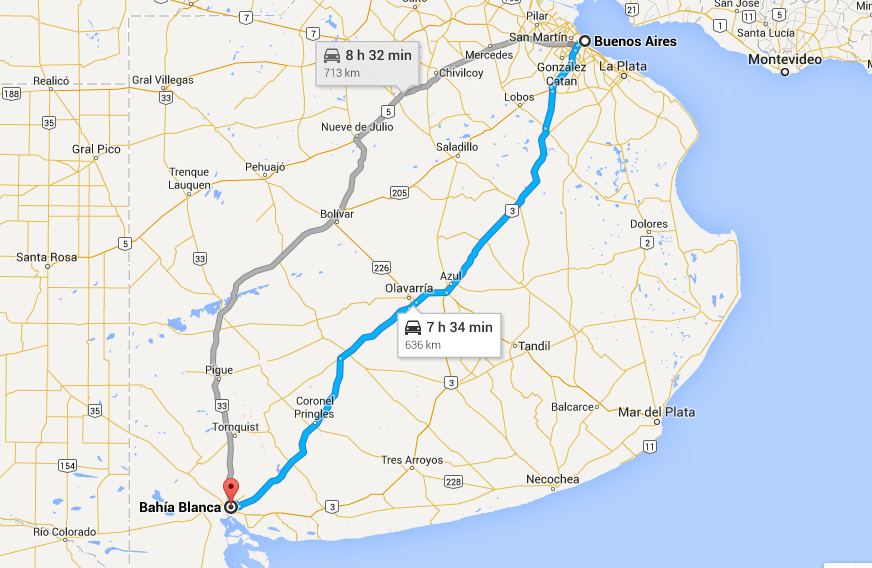
\includegraphics[height=7cm]{google-maps.png} \\
\end{center}
\end{frame}

\begin{frame}{Camino m\'inimo}
\begin{center}
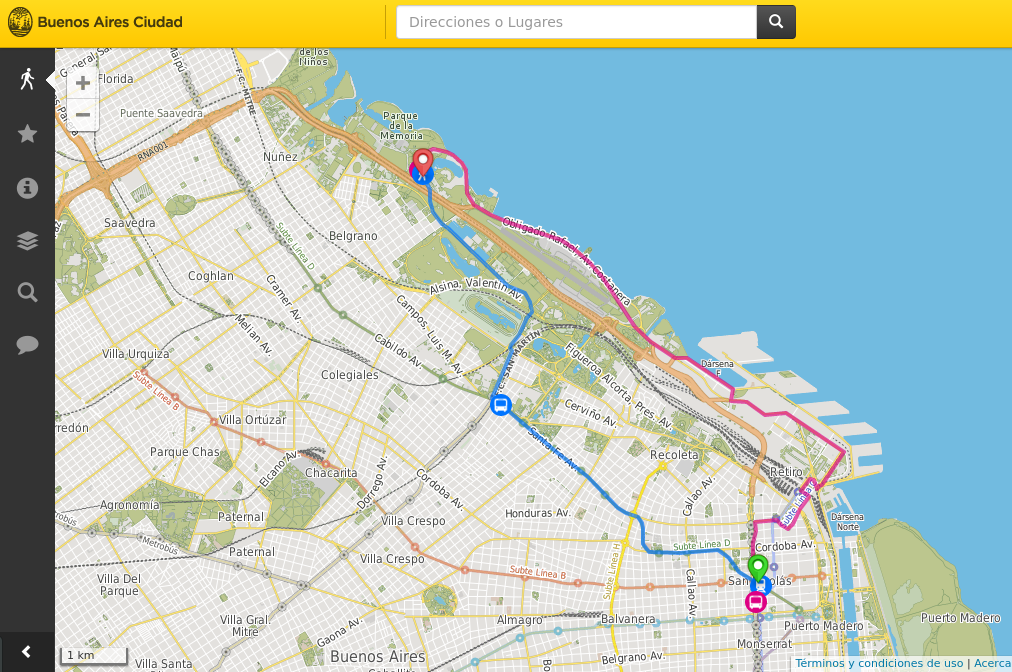
\includegraphics[height=7cm]{mapa-buenos-aires.png} \\
\end{center}
\end{frame}

\begin{frame}{Representando el problema}
Para poder resolver estos problemas debemos poder representarlos de manera
concisa y abstracta, desprendiéndonos de las particularidades de cada
caso de uso posible.

\bigskip

La representación más usual de este tipo de problemas (ya sea para aplicarlo
en problemas de camino mínimo o no) es la de \textbf{grafos}.
\end{frame}

\subsection{Representación con grafos}
\begin{frame}{\textquestiondown Qué es un grafo?}
\begin{exampleblock}{}
  {\large ``Un grafo es un conjunto, no vacío, de objetos llamados vértices 
  (o nodos) y una selección de pares de vértices, llamados aristas 
  (edges en inglés) que pueden ser orientados (dirigidos) o no.''}
  \vskip5mm
  \hspace*\fill{\small--- Wikipedia}
\end{exampleblock}
  \pause
\invisible<1>{
\begin{exampleblock}{}
  {\large ``Un grafo es un conjunto de puntos y líneas que unen pares de esos puntos''}
  \vskip5mm
  \hspace*\fill{\small--- La Posta}
\end{exampleblock}

}
\end{frame}

\begin{frame}{Grafos dirigidos y no dirigidos}

{\small
En los grafos no dirigidos las aristas son doble mano (se puede ir en ambos sentidos). \\
En los dirigidos en cambio, las aristas se recorren en un único sentido: desde el origen al destino de la flecha. Si queremos representar que la calle que une las esquinas $u$ y $v$ es doble mano deberemos poner dos aristas: una que vaya de $u$ a $v$ y otra que vaya de $v$ a $u$.}

\begin{center}
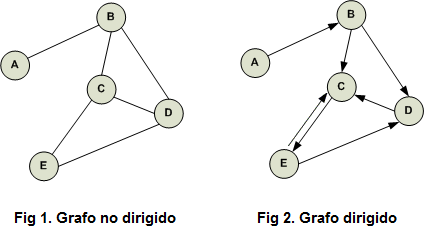
\includegraphics[scale=0.75]{grafos-dirigidos-y-no-dirigidos.png}
\end{center}
\end{frame}

\begin{frame}{\textquestiondown Para qué podemos usar los grafos?}
Mediante un grafo podemos representar, por ejemplo, una ciudad. Las esquinas serían los vértices y las conexiones por medio de una calle entre dos esquinas serían los ejes. Si todas las calles son doble mano, el grafo es no dirigido.
Si algunas calles son mano única el grafo es dirigido: ¿cómo modelamos una calle doble mano aquí?

\bigskip
A medida que los problemas se dificultan, puede suceder que sea difícil que a uno se le ocurra modelar el problema con un grafo, pero que una vez que lo hayamos hecho, el problema se vuelva sencillo utilizando los algoritmos que veremos hoy. 

\end{frame}

\begin{frame}{Formas de representar un grafo}
Existen varias maneras de guardar un grafo en memoria para poder luego consultar cosas (por ejemplo, recorrer el grafo, que es lo que haremos hoy).

Veamos las dos más populares.
\end{frame}

\begin{frame}{Matriz de adyacencia}
\begin{block}{Matriz de adyacencia}
La matriz de adyacencia es una matriz de $n \times n$ donde $n$ es la cantidad de nodos del grafo, que en la posición ($i,j$) tiene un 1 (o true) si hay una arista entre los nodos $i$ y $j$ y 0 (o false) si no.
\end{block}

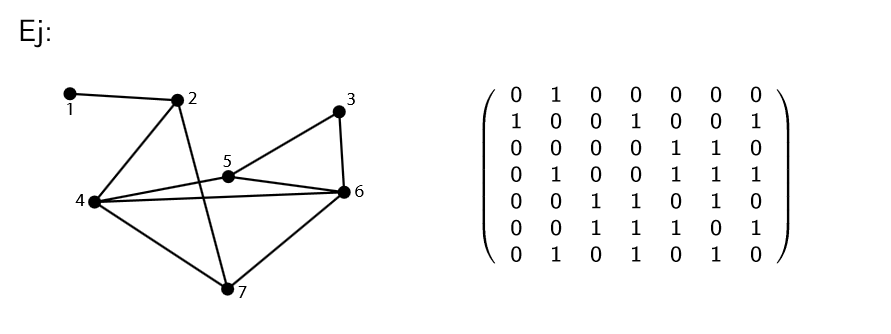
\includegraphics[scale=0.5]{matriz-adyacencia.png}
\end{frame}

\begin{frame}{Matriz de adyacencia}
Esta es una de las representaciones m\'as utilizadas. Si bien el ejemplo es para un grafo no dirigido, tambi\'en se puede utilizar la misma estructura para grafos dirigidos y grafos con pesos.
\bigskip

{\bf Ventajas}
\pause
\invisible<1> {
	\begin{itemize}
		\item Permite saber si existe o no arista entre dos nodos cualesquiera en O(1).
		\item Es muy f\'acil de implementar, $matrizAdy[i][j]$ guarda toda la informaci\'on sobre la arista.
	\end{itemize}
}
\bigpause
{\bf Desventajas}
\pause
\invisible<1> {
	\begin{itemize}
		\item La complejidad espacial: se necesitan $n^2$ casillas para representar un grafo de $n$ nodos.
	\end{itemize}
}
\end{frame}

\begin{frame}{Lista de adyacencia}
\begin{block}{Lista de adyacencia}
La lista de adyacencia es un vector de vectores de enteros, que en el $i$-ésimo vector tiene el número $j$ si hay una arista entre los nodos $i$ y $j$.
\end{block}

Coloquialmente la llamamos {\it lista de vecinos} pues para cada nodo guardamos la lista de nodos para los que existe una arista que los conecta (o sea, los vecinos).
\bigskip
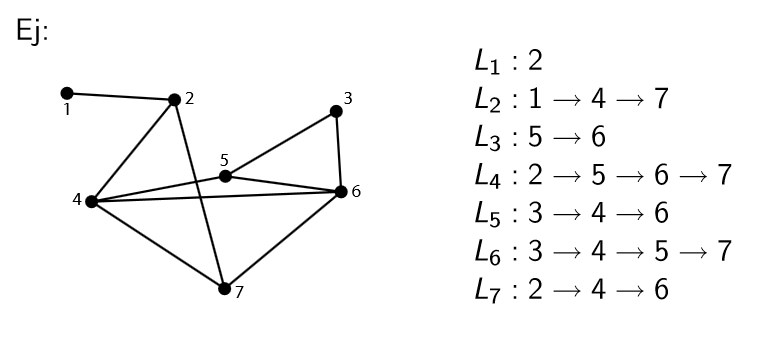
\includegraphics[scale=0.5]{lista-vecinos.png}
\end{frame}

\begin{frame}{Lista de adyacencia}
Nuevamente, con la misma idea tambi\'en se pueden modelar grafos dirigidos y con pesos.\bigskip

La complejidad espacial de esta representaci\'on ser\'a posiblemente mucho menor. ?`Cu\'anta memoria necesitaremos para un grafo de $n$ nodos y $m$ aristas? \pause {\bf O(m+n)}
\end{frame}

\begin{frame}{Formalización del problema de camino mínimo}

Precisemos mejor nuestro problema, usando los términos de grafos que
acabamos de aprender.

\begin{block}{Problema de Camino m\'inimo}
Dado un grafo $G$ con pesos en las aristas, el problema de
camino mínimo entre dos nodos $u$ y $v$ consiste en encontrar un camino
entre esos nodos cuyo peso sea menor o igual que el peso de cualquier
otro camino entre $u$ y $v$.
\end{block}

\bigskip

Según qué tipo de grafo analicemos, la solución al problema será diferente.
Por ejemplo, si el grafo no tuviera pesos (o si todos los pesos fueran iguales,
que a efectos prácticos es lo mismo), nos conviene usar otro algoritmo (BFS).

\end{frame}

\subsection{Algoritmo de Dijkstra}
\begin{frame}{Algoritmo de Dijkstra}
Este algoritmo fue creado por uno de los padres de la computación,
Edger W. Dijkstra, en 1956. Sirve para cualquier grafo con pesos (dirigido
o no) \textbf{siempre y cuando sus pesos no sean negativos}.

\end{frame}

\begin{frame}{Idea del algoritmo de Dijkstra}
\begin{itemize}
\item El algoritmo calcula las distancias mínimas desde un nodo inicial a todos 
los demás. Para hacerlo, en cada paso se toma el nodo más cercano al inicial
que aún no fue visitado (le diremos $v$). Este nodo tiene calculada la menor distancia
al nodo inicial (\textquestiondown por qué?). 
\item Luego, recalculamos todas los caminos mínimos, teniendo en cuenta a 
$v$ como camino intermedio.
\item Así, en cada paso tendremos un subconjunto de nodos que ya tienen calculada
su mínima distancia y los demás tienen calculada su mínima distancia si solo
puedo usar los nodos del conjunto como nodos intermedios. 
\item Con cada iteración agregaremos un nodo más a nuestro conjunto, hasta resolver el 
problema en su totalidad.
\end{itemize}

Veamos un ejemplo.
\end{frame}


\begin{frame}{Algoritmo de Dijkstra - Ejemplo}

\begin{pgfpicture}{0cm}{0cm}{11cm}{7cm}
	\pgfsetlinewidth{1pt}
	\pgfnodecircle{v1}[stroke]{\pgfxy(2,3)}{2mm}			
	\pgfputat{\pgfxy(2,3)}{\pgfbox[center,center]{1}}
	\pgfnodecircle{v2}[stroke]{\pgfxy(4,5)}{2mm}
	\pgfputat{\pgfxy(4,5)}{\pgfbox[center,center]{2}}
	\pgfnodecircle{v3}[stroke]{\pgfxy(7,5)}{2mm}
	\pgfputat{\pgfxy(7,5)}{\pgfbox[center,center]{3}}
	\pgfnodecircle{v4}[stroke]{\pgfxy(9,3)}{2mm}
	\pgfputat{\pgfxy(9,3)}{\pgfbox[center,center]{4}}
	\pgfnodecircle{v5}[stroke]{\pgfxy(7,1)}{2mm}
	\pgfputat{\pgfxy(7,1)}{\pgfbox[center,center]{5}}
	\pgfnodecircle{v6}[stroke]{\pgfxy(4,1)}{2mm}
	\pgfputat{\pgfxy(4,1)}{\pgfbox[center,center]{6}}
	\pgfnodesetsepend{3pt}
	\pgfsetarrowsend{latex}
    	\pgfnodeconnline{v1}{v2}
	\pgfnodeconnline{v1}{v6}			
	\pgfnodeconnline{v1}{v3}			
	\pgfnodelabel{v1}{v2}[0.5][5pt]{\pgfbox[center,center]{4}}			
	\pgfnodeconnline{v2}{v3}
	\pgfnodelabel{v2}{v3}[0.5][5pt]{\pgfbox[center,center]{3}}						
	\pgfnodeconnline{v3}{v4}
	\pgfnodelabel{v3}{v4}[0.5][5pt]{\pgfbox[center,center]{1}}						
	\pgfnodeconnline{v5}{v4}
	\pgfnodelabel{v5}{v4}[0.5][5pt]{\pgfbox[center,center]{4}}						
	\pgfnodeconnline{v6}{v5}			
	\pgfnodelabel{v6}{v5}[0.5][5pt]{\pgfbox[center,center]{3}}			
	\pgfnodelabel{v1}{v6}[0.5][5pt]{\pgfbox[center,center]{3}}			
	\pgfnodelabel{v1}{v3}[0.5][5pt]{\pgfbox[center,center]{7}}			
	\pgfnodeconnline{v2}{v5}			
	\pgfnodelabel{v2}{v5}[0.5][5pt]{\pgfbox[center,center]{1}}			
	\pgfnodeconnline{v3}{v5}			
	\pgfnodelabel{v3}{v5}[0.5][5pt]{\pgfbox[center,center]{1}}			
	
	\onslide<2-2>{
		\pgfputat{\pgfxy(5,7)}{\pgfbox[left,top]{$\pi=(0,\infty,\infty,\infty,\infty,\infty)$}}
	}
	\onslide<2-3>{
		\pgfputat{\pgfxy(1,7)}{\pgfbox[left,top]{$S=\{1\}$}}
	}
	
	\color{orange}
	\onslide<2->{
		\pgfnodecircle{v1}[stroke]{\pgfxy(2,3)}{2mm}			
	}
	
	\color{black}
	\onslide<3-5>{
	   \pgfputat{\pgfxy(5,7)}{\pgfbox[left,top]{$\pi=(0,4,7,\infty,\infty,3)$}}
	}
	
	\onslide<3->{
		\color{darkgreen}
		\pgfnodeconnline{v1}{v2}
		\pgfnodeconnline{v1}{v6}			
		\pgfnodeconnline{v1}{v3}
	}
	
	\color{black}
	\onslide<4-6>{
		\pgfputat{\pgfxy(1,7)}{\pgfbox[left,top]{$S=\{1,6\}$}}
	}
	
	\color{orange}
	\onslide<4->{
		\pgfnodecircle{v6}[stroke]{\pgfxy(4,1)}{2mm}			
		\pgfnodeconnline{v1}{v6}			
	}
	
	\color{blue}
	\onslide<5-5>{
		\pgfnodeconnline{v6}{v5}
	}
	
	\color{black}
	\onslide<6-8>{
	  \pgfputat{\pgfxy(5,7)}{\pgfbox[left,top]{$\pi=(0,4,7,\infty,6,3)$}}
	}
	
	\color{darkgreen}
	\onslide<6-8>{
		\pgfnodeconnline{v6}{v5}
	}
	
	\color{black}		
	\onslide<7-9>{
		\pgfputat{\pgfxy(1,7)}{\pgfbox[left,top]{$S=\{1,6,2\}$}}
	}
	
	\color{orange}
	\onslide<7->{
		\pgfnodecircle{v2}[stroke]{\pgfxy(4,5)}{2mm}			
		\pgfnodeconnline{v1}{v2}
	}
	
	\color{blue}
	\onslide<8-8>{
		\pgfnodeconnline{v2}{v3}
		\pgfnodeconnline{v2}{v5}
	}
	
	\color{darkgreen}
	\onslide<9-11>{
		\pgfnodeconnline{v2}{v5}
		\color{black}
		\pgfputat{\pgfxy(5,7)}{\pgfbox[left,top]{$\pi=(0,4,7,\infty,5,3)$}}
	}
	
	\color{black}
	\onslide<10-12>{
		\pgfputat{\pgfxy(1,7)}{\pgfbox[left,top]{$S=\{1,6,2,5\}$}}
	}

	\color{orange}
	\onslide<10->{
		\pgfnodecircle{v5}[stroke]{\pgfxy(7,1)}{2mm}			
		\pgfnodeconnline{v2}{v5}
	}
	
	\color{blue}
	\onslide<11-11>{
		\pgfnodeconnline{v5}{v4}
	}
	
	\color{black}
	\onslide<12-14>{
		\pgfputat{\pgfxy(5,7)}{\pgfbox[left,top]{$\pi=(0,4,7,9,5,3)$}}
		\color{darkgreen}
		\pgfnodeconnline{v5}{v4}
	}
	
	\color{black}
	\onslide<13-15>{
		\pgfputat{\pgfxy(1,7)}{\pgfbox[left,top]{$S=\{1,6,2,5,3\}$}}
	}

	\color{orange}
	\onslide<13->{
		\pgfnodecircle{v3}[stroke]{\pgfxy(7,5)}{2mm}			
		\pgfnodeconnline{v1}{v3}
	}
	
	\color{blue}
	\onslide<14-14>{
		\pgfnodeconnline{v3}{v4}
	}
	
	\color{black}
	\onslide<15->{
		\pgfputat{\pgfxy(5,7)}{\pgfbox[left,top]{$\pi=(0,4,7,8,5,3)$}}
		\color{darkgreen}
		\pgfnodeconnline{v3}{v4}
	}
	
	\onslide<16->{
	  \color{black}
		\pgfputat{\pgfxy(1,7)}{\pgfbox[left,top]{$S=\{1,6,2,5,3,4\}$}}
	}

	\color{orange}
	\onslide<16->{
		\pgfnodecircle{v4}[stroke]{\pgfxy(9,3)}{2mm}			
		\pgfnodeconnline{v3}{v4}
	}
\end{pgfpicture}
\end{frame}

\subsection{\textquestiondown Por qué funciona este algoritmo?}
\begin{frame}{\textquestiondown Por qué funciona este algoritmo?}
Si bien no veremos la demostración formal, la clave está en que:

\begin{itemize}
\item En cada paso, para todos los nodos $u$ que ya fueron visitados,
el algoritmo tiene calculada la mínima distancia del nodo inicial a $u$.
Para los nodos $v$ que aún no fueron visitados, el algoritmo tiene calculada
la distancia mínima si solo podemos utilizar nodos ya visitados como puntos
intermedios del camino.
\item El próximo nodo a ser visitado es el más cercano al nodo inicial
que aún no fue visitado. Entonces, este ya tiene calculada la distancia
correcta (si no, habría una mejor solución usando nodos no visitados como
nodos intermedios, pero este nodo es el más cercano al origen entre todos los
no visitados!).
\item Al comienzo, las distancias están bien calculadas.
\end{itemize}

\end{frame}

\begin{frame}[fragile]{Pseudocódigo de Dijkstra sin cola de prioridad}
\begin{lstlisting}
Dijkstra (Grafo G, nodo inicial s)
  visitado[n] = {false, ..., false} // guarda si un nodo ya fue visitado
  distancia[n] = {Infinito, ..., Infinito} // guarda las distancias del nodo salida al resto
  
  para cada w en V[G] hacer
     si existe arista entre s y w entonces
         distancia[w] = peso (s, w)

  distancia[s] = 0
  visitado[s] = true
  
  mientras que no esten visitados todos hacer 
     v = nodo de menor distancia a s que no fue visitado aun
     visitado[v] = true
     para cada w en sucesores (G, v) hacer
         si distancia[w] > distancia[v] + peso (v, w) entonces
            distancia[w] = distancia[v] + peso (v, w)
            padre[w] = v

\end{lstlisting}
\end{frame}

\begin{frame}{Costo de esta implementación de Dijkstra}
Podemos ver que utiliza $O(n^2)$ operaciones, siendo $n$ la cantidad de
nodos del problema.
\end{frame}

\begin{frame}{Otra implementación}
Existen otras implementaciones del algoritmo de Dijkstra. La que veremos
a continuación solo difiere de la anterior en la forma de guardar los
nodos candidatos a ser visitados.
\end{frame}

\begin{frame}[fragile]{Pseudocódigo de Dijkstra con cola de prioridad}
\begin{lstlisting}
Dijkstra (Grafo G, nodo_fuente s)       
   para todo u en V[G] hacer
       distancia[u] = INFINITO
       padre[u] = NULL
       visitado[u] = false
       
   distancia[s] = 0
   adicionar (cola, (s, distancia[s]))
   
   mientras que cola no sea vacia hacer
       u = extraer_minimo(cola)
       visitado[u] = true
       para todo v en adyacencia[u] hacer
           si no visitado[v] y distancia[v] > distancia[u] + peso (u, v) hacer
              distancia[v] = distancia[u] + peso (u, v)
              padre[v] = u
              adicionar(cola,(v, distancia[v]))
\end{lstlisting}
\end{frame}

\begin{frame}{Costo de esta implementación de Dijkstra}
Podemos ver que utiliza $O(m \log n)$ operaciones, siendo $n$ la cantidad de
nodos del problema y $m$ la cantidad de aristas. No veremos hoy la demostración,
pero se basa en que las estructuras que usamos para la cola de prioridad
extraen e insertan un elemento en tiempo logarítmico.

\bigskip

Existen varias estructuras en C++ para implementar cola de prioridad. Dos
ejemplos son \texttt{priority\_queue} y \texttt{set}.

\end{frame}

\begin{frame}{\textquestiondown Qué implementación uso?}
\begin{itemize}
\item Si el grafo es \textbf{ralo}, o sea, tiene pocas aristas, conviene utilizar 
\\ \pause \invisible<1> { la implementación con cola de prioridad ($O(m \log n)$) 
\pause \invisible<1-2> { 
\item Si el grafo es \textbf{denso}, o sea, tiene muchas aristas, conviene 
utilizar \pause \invisible<1-3> { la implementación básica ($O(n^2)$) } } } 
\end{itemize} 
\end{frame}

\subsection{Camino mínimo en una grilla}
Hallemos el camino mínimo entre dos casillas $(a,b)$ y $(c,d)$ de una matriz de $m \times n$.
Al programar nos puede servir usar los siguientes trucos de los que hablaremos:

\begin{frame}
\begin{itemize}
\item Vector de movimientos (dx, dy)
\item Representar una dirección (0, 1, 2, 3 en los arreglos de arriba) y un giro (sumar mod 4)
\item Bordes (hacer padding)
\end{itemize}
\end{frame}

\section{Árbol generador mínimo}

\subsection{\textquestiondown Qué es un árbol generador mínimo?}

\begin{frame}{\textquestiondown Qué es un árbol?}
\begin{block}{Árboles}
Un árbol es un tipo especial de grafo no dirigido. Es un grafo donde 
entre cualquier par de nodos existe un único camino que los conecta 
(notar que en particular, todos los nodos tienen que estar conectados entre sí).
\end{block}

Los árboles tienen mil propiedades interesantes, como $m = n -1$, 
que no tiene ciclos y más cosas sobre las que hoy no hablaremos.
\end{frame}

\begin{frame}{\textquestiondown Qué es un árbol generador mínimo?}

Un \textbf{árbol generador mínimo} es un árbol que utiliza todos los nodos
del grafo, de manera tal que el costo total de sumar las aristas del grafo
es mínimo.

\bigskip

Veamos un ejemplo.
\end{frame}

\begin{frame}{Ejemplo de árbol generador mínimo}
\begin{center}
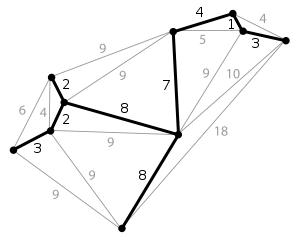
\includegraphics[height=7cm]{mst.png} \\
\end{center}
\end{frame}

\begin{frame}{\textquestiondown Para qué sirve encontrar un árbol generador mínimo?}
Este problema es muy relevante, porque en diversas situaciones hallarlo
resuelve nuestro problema. Muchas veces, a simple vista no es nada obvio
que se resuelve con esto.

\bigskip

En un país con muchas ciudades, nos piden que creemos rutas de manera tal que
se pueda viajar de cualquier ciudad a cualquier otra usando la menor cantidad
de dinero posible. Para algunos pares de ciudades (que son las ciudades entre las
que tenemos permitido crear una ruta) sabemos el costo de crear una ruta entre ellos.
\textquestiondown Qué rutas deberíamos construir para lograr el objetivo?

\end{frame}

\subsection{Algoritmo de Prim}
\begin{frame}

\begin{itemize}
\item El algoritmo de Prim mantiene un conjunto de nodos $C$ que son los nodos que
ya fueron conectados entre sí. 
\item En cada paso, elige la arista más barata entre algún nodo de $C$ y un 
nodo no agregado todavía. Al elegir la arista, se agrega el nodo nuevo a $C$. 
\item De esta forma, en cada paso hay un nodo nuevo sumándose al 
conjunto de nodos ya conectados entre sí. 
\item Luego de $n-1$ pasos, habremos agregado todos los nodos de la forma más
barata posible: obtendremos un árbol generador mínimo.
\end{itemize}

\end{frame}


\begin{frame}{Algoritmo de Prim - Ejemplo}

\begin{pgfpicture}{0cm}{0cm}{11cm}{7cm}
	\pgfsetlinewidth{1pt}
	\pgfnodecircle{v1}[stroke]{\pgfxy(2,3)}{2mm}			
	\pgfputat{\pgfxy(2,3)}{\pgfbox[center,center]{1}}
	\pgfnodecircle{v2}[stroke]{\pgfxy(4,5)}{2mm}
	\pgfputat{\pgfxy(4,5)}{\pgfbox[center,center]{2}}
	\pgfnodecircle{v3}[stroke]{\pgfxy(7,5)}{2mm}
	\pgfputat{\pgfxy(7,5)}{\pgfbox[center,center]{3}}
	\pgfnodecircle{v4}[stroke]{\pgfxy(9,3)}{2mm}
	\pgfputat{\pgfxy(9,3)}{\pgfbox[center,center]{4}}
	\pgfnodecircle{v5}[stroke]{\pgfxy(7,1)}{2mm}
	\pgfputat{\pgfxy(7,1)}{\pgfbox[center,center]{5}}
	\pgfnodecircle{v6}[stroke]{\pgfxy(4,1)}{2mm}
	\pgfputat{\pgfxy(4,1)}{\pgfbox[center,center]{6}}
	\pgfnodesetsepend{3pt}
	%\pgfsetarrowsend{Triangle[scale=0.7pt]}
    	\pgfnodeconnline{v1}{v2}
	\pgfnodeconnline{v1}{v6}			
	\pgfnodeconnline{v1}{v3}			
	\pgfnodelabel{v1}{v2}[0.5][5pt]{\pgfbox[center,center]{4}}			
	\pgfnodeconnline{v2}{v3}
	\pgfnodelabel{v2}{v3}[0.5][5pt]{\pgfbox[center,center]{3}}						
	\pgfnodeconnline{v3}{v4}
	\pgfnodelabel{v3}{v4}[0.5][5pt]{\pgfbox[center,center]{1}}						
	\pgfnodeconnline{v5}{v4}
	\pgfnodelabel{v5}{v4}[0.5][5pt]{\pgfbox[center,center]{4}}						
	\pgfnodeconnline{v6}{v5}			
	\pgfnodelabel{v6}{v5}[0.5][5pt]{\pgfbox[center,center]{3}}			
	\pgfnodelabel{v1}{v6}[0.5][5pt]{\pgfbox[center,center]{3}}			
	\pgfnodelabel{v1}{v3}[0.5][5pt]{\pgfbox[center,center]{7}}			
	\pgfnodeconnline{v2}{v5}			
	\pgfnodelabel{v2}{v5}[0.5][5pt]{\pgfbox[center,center]{1}}			
	\pgfnodeconnline{v3}{v5}			
	\pgfnodelabel{v3}{v5}[0.5][5pt]{\pgfbox[center,center]{1}}			
	
	\onslide<2-2>{
		\pgfputat{\pgfxy(5,7)}{\pgfbox[left,top]{$\pi=(0,\infty,\infty,\infty,\infty,\infty)$}}
	}
	\onslide<2-3>{
		\pgfputat{\pgfxy(1,7)}{\pgfbox[left,top]{$S=\{1\}$}}
	}
	
	\color{orange}
	\onslide<2->{
		\pgfnodecircle{v1}[stroke]{\pgfxy(2,3)}{2mm}			
	}
	
	\color{black}
	\onslide<3-5>{
	   \pgfputat{\pgfxy(5,7)}{\pgfbox[left,top]{$\pi=(0,4,7,\infty,\infty,3)$}}
	}
	
	\onslide<3->{
		\color{darkgreen}
		\pgfnodeconnline{v1}{v6}			
		\pgfnodeconnline{v1}{v3}
	}

	\onslide<3-10>{
		\color{darkgreen}
		\pgfnodeconnline{v1}{v3}
	}

	\onslide<3-12>{
		\color{darkgreen}
		\pgfnodeconnline{v1}{v2}
	}
	
	\color{black}
	\onslide<4-6>{
		\pgfputat{\pgfxy(1,7)}{\pgfbox[left,top]{$S=\{1,6\}$}}
	}
	
	\color{orange}
	\onslide<4->{
		\pgfnodecircle{v6}[stroke]{\pgfxy(4,1)}{2mm}			
		\pgfnodeconnline{v1}{v6}			
	}
	
	\color{blue}
	\onslide<5-5>{
		\pgfnodeconnline{v6}{v5}
	}
	
	\color{black}
	\onslide<6-8>{
	  \pgfputat{\pgfxy(5,7)}{\pgfbox[left,top]{$\pi=(0,4,7,\infty,6,3)$}}
	}
	
	\color{darkgreen}
	\onslide<6-8>{
		\pgfnodeconnline{v6}{v5}
	}
	
	\color{black}		
	\onslide<7-9>{
		\pgfputat{\pgfxy(1,7)}{\pgfbox[left,top]{$S=\{1,6,2\}$}}
	}
	
	\color{orange}
	\onslide<7->{
		\pgfnodecircle{v5}[stroke]{\pgfxy(7,1)}{2mm}
		\pgfnodeconnline{v6}{v5}
	}
	
	\color{blue}
	\onslide<8-8>{
		\pgfnodeconnline{v5}{v4}
		\pgfnodeconnline{v5}{v2}
		\pgfnodeconnline{v5}{v3}
	}
	
	\color{darkgreen}
	\onslide<9-12>{
		\pgfnodeconnline{v5}{v4}
		\pgfnodeconnline{v5}{v2}
		\pgfnodeconnline{v5}{v3}
		\color{black}
		\pgfputat{\pgfxy(5,7)}{\pgfbox[left,top]{$\pi=(0,4,7,\infty,5,3)$}}
	}
	
	\color{black}
	\onslide<10-12>{
		\pgfputat{\pgfxy(1,7)}{\pgfbox[left,top]{$S=\{1,6,2,5\}$}}
	}

	\color{orange}
	\onslide<10->{
		\pgfnodecircle{v3}[stroke]{\pgfxy(7,5)}{2mm}		
		\pgfnodeconnline{v5}{v3}
	}
	
	\color{blue}
	\onslide<11-11>{
		\pgfnodeconnline{v2}{v3}
		\pgfnodeconnline{v3}{v4}
	}

	\color{red}
	\onslide<11-11>{
		\pgfnodeconnline{v1}{v3}
	}

	\color{darkgreen}
	\onslide<12-14>{
		\pgfnodeconnline{v2}{v3}
		\pgfnodeconnline{v3}{v4}
		\pgfnodeconnline{v1}{v2}
	}

	\color{black}
	\onslide<12->{
		\pgfnodeconnline{v1}{v3}
	}
	
	\color{black}
	\onslide<12-14>{
		\pgfputat{\pgfxy(5,7)}{\pgfbox[left,top]{$\pi=(0,4,7,9,5,3)$}}
		\color{darkgreen}
		\pgfnodeconnline{v5}{v4}
	}
	
	\color{black}
	\onslide<13-15>{
		\pgfputat{\pgfxy(1,7)}{\pgfbox[left,top]{$S=\{1,6,2,5,3\}$}}
	}

	\color{orange}
	\onslide<13->{
		\pgfnodecircle{v2}[stroke]{\pgfxy(4,5)}{2mm}			
		\pgfnodeconnline{v5}{v2}
	}
	
	\color{red}
	\onslide<14-14>{
		\pgfnodeconnline{v1}{v2}
		\pgfnodeconnline{v2}{v3}
	}
	
	\color{darkgreen}
	\onslide<15-15>{
		\pgfnodeconnline{v3}{v4}
		\pgfnodeconnline{v4}{v5}
	}

	\color{orange}
	\onslide<16->{
		\pgfnodecircle{v4}[stroke]{\pgfxy(9,3)}{2mm}			
		\pgfnodeconnline{v3}{v4}
	}
\end{pgfpicture}
\end{frame}

\begin{frame}[fragile]{Pseudocódigo de Prim sin cola de prioridad}
\begin{lstlisting}
Prim (Grafo G, nodo inicial s)
  visitado[n] = {false, ..., false} // guarda si un nodo ya fue visitado
  distancia[n] = {Infinito, ..., Infinito} // guarda las distancias de cada nodo al conjunto visitado
  
  para cada w en V[G] hacer
     si existe arista entre s y w entonces
         distancia[w] = peso (s, w)

  distancia[s] = 0
  visitado[s] = true
  mientras que no esten visitados todos hacer 
     v = nodo de menor distancia del conjunto que no fue visitado aun (itero el arreglo)
     visitado[v] = true
     para cada w en los vecinos de v hacer
         si distancia[w] > peso (v, w) entonces
            distancia[w] = peso (v, w)
            padre[w] = v
\end{lstlisting}
\end{frame}

\begin{frame}[fragile]{Pseudocódigo de Prim con cola de prioridad}
\begin{lstlisting}
Prim (Grafo G, nodo_fuente s)       
   para todo u en V[G] hacer
       distancia[u] = INFINITO
       padre[u] = NULL
       visitado[u] = false
       
   distancia[s] = 0
   adicionar (cola, (distancia[s], s))
   
   mientras que cola no sea vacia hacer
       u = extraer_minimo(cola)
       visitado[u] = true
       para todo v en vecinos de u hacer
           si no visitado[v] y distancia[v] > peso(u, v) hacer
              distancia[v] = peso(u, v)
              padre[v] = u
              adicionar(cola, (distancia[v], v))
\end{lstlisting}
\end{frame}


\begin{frame}
\begin{center}
{\Huge \textquestiondown Preguntas?}
\end{center}
\end{frame}

\end{document}
